% !TEX program = xelatex
\documentclass[11pt,a4paper]{article}
\usepackage{fontspec}
\setmainfont{DejaVuSerif}[Path=fonts/,Extension=.ttf,
  BoldFont=DejaVuSerif-Bold,ItalicFont=DejaVuSerif-Italic,
  BoldItalicFont=DejaVuSerif-BoldItalic]
\setmonofont{DejaVuSansMono}[Path=fonts/,Extension=.ttf,Scale=.86]
\usepackage[english,russian]{babel}
\usepackage[margin=22mm]{geometry}
\usepackage{amsmath,amssymb,booktabs,tabularx,longtable,array}
\usepackage{graphicx,xcolor,caption,enumitem,fancyhdr}
\usepackage[unicode,hidelinks]{hyperref}
\usepackage{microtype}
\graphicspath{{images/}}
\setlength{\parindent}{0pt}
\setlength{\parskip}{5pt}
\setlength{\emergencystretch}{2em}
\renewcommand{\arraystretch}{1.15}
\captionsetup{font=small,labelfont=bf}
\setlist{nosep,leftmargin=*}
\pagestyle{fancy}
\fancyhf{}
\fancyhead[L]{\small Генерация кода с нуля}
\fancyhead[R]{\small NLP · ДЗ 2}
\fancyfoot[C]{\thepage}
\setlength{\headheight}{14pt}
\newcommand{\pass}{\textnormal{pass@1}}
\newcommand{\loss}{\textnormal{token loss}}
\newcommand{\code}[1]{\texttt{\detokenize{#1}}}
\newcommand{\pending}[1]{\textcolor{blue!60!black}{#1}}
\newcolumntype{Y}{>{\raggedright\arraybackslash}X}
\setcounter{tocdepth}{1}
\title{\textbf{Генерация Python-кода по тексту задачи}\\
\large Обучение encoder--decoder Transformer с нуля}
\author{}
\date{Рабочий черновик 0.4 · 23 октября 2026}
\begin{document}
\maketitle
\begin{abstract}
Исследуется генерация Python-программы по условию арифметической задачи.
Путь к решению включает baseline на основе BART, увеличение модели,
диагностику нестабильного обучения, короткий поиск архитектуры,
сравнение T5-style и pointer-generator, а также проверку разнообразия
данных и параметров beam search. В сопоставимом бюджете четырёх миллионов
предъявлений BART на различных train-примерах получил 68.6765\% локального
\pass{} против 67.6104\% при повторении одного миллиона примеров.
Выбранный BART 8+8/d1024 затем обучен с нуля на полном подготовленном train
за четыре эпохи; лучший validation \loss{} составил 0.191021.
На прежней фиксированной validation полная модель получила 74.2985\%
\pass{} (+5.6220 п.п. к короткой Distinct4m). На одной NVIDIA T4
генерация всех 1919 официальных ответов заняла 165.1 секунды при beam 4,
то есть уложилась в лимит 180 секунд. Однако на public-половине
официального теста новая модель получила 729/960 = 75.94\%
против 735/960 = 76.56\% у прежней полной модели 002:
на шесть решений меньше ($-0.625$ п.п.). Результат private пока неизвестен.
\end{abstract}
{\small\textbf{Статус документа.} Черновик по сохранённым
результатам, дополненный оценкой полной модели, замером T4
и сравнением двух официальных public-посылок.
Работа с моделью продолжается отдельно; здесь фиксируются уже
проверенные наблюдения. Текст, таблицы и рисунки будем уточнять по разделам.}
{\small\tableofcontents}
\newpage
\section{Задача и данные}

\subsection{Постановка}
По текстовому условию нужно сгенерировать Python-код с функцией
\code{solve()}, возвращающей ответ. По правилам задания модель обучается
с нуля и имеет Transformer-энкодер и декодер. Все ответы официального
теста должны генерироваться за 180 секунд на одной NVIDIA T4;
дополнительные обучающие данные и таргеты запрещены~\cite{assignment}.
Также я учитывал отдельный запрет спекулятивного декодирования.

Цель экспериментов --- выбрать конфигурацию, которая сочетает качество
решений, устойчивое обучение и приемлемую стоимость генерации.
Названия BART и T5 далее обозначают устройство моделей:
предобученные веса не использовались.

\subsection{Подготовка и разбиения}
Использован корпус \code{SlavaYus/tinysms_qa_12m}: в исходном train
11\,838\,003 пары \code{question}/\code{code}, официальный test содержит
1919 условий без кода~\cite{dataset}. Комментарии в коде удалялись
Python-токенизатором с сохранением строковых литералов и структуры
программы. Длинные обучающие пары исключались целиком, а не обрезались.

Первые эксперименты использовали разбиение 80/10/10 с seed 42.
Начиная с модели 002 использовалось 98/1/1. После фильтрации по лимитам
256 токенов осталось 11\,593\,060 train и 118\,302 validation.
Новый внутренний test выделен отдельно из исходного train.
Официальный test при обучении и подборе параметров не использовался.

\begin{table}[htbp]
\centering\small
\begin{tabularx}{\linewidth}{lXr}
\toprule
Обозначение & Назначение & Размер \\
\midrule
Test-001 & Выборка из test разбиения 80/10/10 & 10\,000 \\
Test-002 & Выборка из нового test разбиения 98/1/1 & 10\,000 \\
Val-20k & Фиксированная validation коротких сравнений & 20\,000 \\
Val-full & Полная validation моделей 002/003 и нового BART & 118\,302 \\
Official & Официальный test без открытых эталонов & 1919 \\
\bottomrule
\end{tabularx}
\caption{Наборы с разными назначениями. Test-001 и Test-002 нельзя считать
одной выборкой, хотя оба содержат 10\,000 строк.}
\label{tab:splits}
\end{table}

Для короткого поиска взяты фиксированные 1\,000\,000 train и Val-20k.
В последующем сравнении данных использовались повторение этого миллиона
четыре раза либо четыре миллиона различных исходных train-строк.
Полный новый BART использовал прежний токенизированный кэш целиком:
порядок строк и исходные таргеты сохранены, ретокенизация не выполнялась.

Разбиение выполнено по строкам. Группировка одинаковых условий между
частями не реализована, поэтому возможны повторы и зависимые примеры.
Отдельно учтено, что старый Test-001 после перехода к 98/1/1 уже
не является гарантированно отложенной выборкой для модели 002.

\subsection{Токенизатор}
Обучен собственный byte-level BPE со словарём 8000 токенов на разрешённых
train-текстах; готовый словарь другой модели не загружался.
Байтовое представление сохраняет отступы и переводы строк программы.
Спецтокены: PAD, UNK, BOS и EOS с ID 0, 1, 2, 3.
В labels нет начального BOS, padding заменён на $-100$;
декодер начинает генерацию с BOS и заканчивает по EOS либо лимиту длины.
В сравнениях архитектур использован один и тот же сохранённый BPE.

\section{Модели, обучение и измерения}

\subsection{Архитектуры}
Основная реализация использует BART encoder--decoder из Transformers,
инициализированный случайно~\cite{bart}. Энкодер получает условие,
декодер --- предыдущие токены программы с причинной маской.
Embeddings энкодера, декодера и выходной проекции связаны.
Обозначение E+D далее задаёт число слоёв энкодера и декодера.

\begin{table}[htbp]
\centering\small
\begin{tabularx}{\linewidth}{lrrrX}
\toprule
Модель & E+D & $d$ & FFN & Особенности \\
\midrule
Baseline-001 & 6+6 & 512 & 2048 & BART, 8 heads \\
Transformer-002 & 8+8 & 768 & 3072 & 139.25 млн параметров \\
Transformer-003 & 10+10 & 1024 & 4096 & 303.18 млн параметров \\
BART-кандидат & 8+8 & 1024 & 4096 & 244.39 млн параметров \\
T5-style & 8+8 & 1024 & 2816 & GEGLU, Pre-RMSNorm, relative bias \\
Copy & 8+8 & 1024 & 4096 & BART и отдельная copy attention \\
\bottomrule
\end{tabularx}
\caption{Основные архитектуры. Различия глубины в коротком поиске
дополнительно приведены в таблице~\ref{tab:h100}.}
\end{table}

T5-style использует относительный attention bias с 32 buckets,
GEGLU и связанные embeddings; число параметров --- 247\,310\,848.
Вариант вдохновлён семейством T5~\cite{t5}, но не воспроизводит полностью
рецепт T5 v1.1: здесь сохранены dropout 0.1 и tied embeddings.
У BART attention dropout равен 0.0, поэтому сравнение затрагивает
весь набор архитектурных настроек, а не одну нормализацию.

В Copy к BART добавлено распределение копирования по токенам условия.
Идея pointer-generator~\cite{pointer} реализована как смесь
\[
 p(y_t\mid x,y_{<t})=g_t\,p_{\mathrm{vocab}}(y_t)
 +(1-g_t)\sum_{i:x_i=y_t}a_{ti}.
\]
Повторяющиеся токены входа суммируются, специальные и masked токены
исключаются. При отсутствии допустимых токенов используется словарь.
Дополнительные метки копирования не нужны; обучение использует прежний код.
Число параметров Copy --- 244\,656\,129.


\subsection{Обучение и функции потерь}
Модель обучалась с teacher forcing и кросс-энтропией следующего токена.
Для сравнения использовалась token-normalized validation loss:
\[
 L_{\mathrm{token}}=
 -\frac{\sum_{i}\sum_{t\in T_i}\log p_\theta(y_{it}\mid x_i,y_{i,<t})}
 {\sum_i |T_i|},
\]
где $T_i$ содержит целевые токены без padding. Обычный \code{eval_loss}
Trainer усредняется иначе и не подменяет эту величину.
Train loss в графиках --- сохранённое среднее по интервалу логирования;
поэтому его значения не следует трактовать как ту же оценку, что
validation loss, рассчитанный по всем целевым токенам.

В основных поздних опытах использовались AdamW, weight decay 0.01,
clipping 1.0, warmup первых 5\% шагов и cosine decay.
Случайная инициализация и выборки закреплены seed 42.
Смешанная точность выбиралась по GPU: BF16 на части запусков A100/H100,
FP16 на T4 и в итоговом A100-запуске. Конкретные LR, batch и бюджет
указаны у соответствующих экспериментов.

При FP16 GradScaler может пропустить обновление и уменьшить scale.
Поэтому для новых запусков различаются плановые попытки шага Trainer
и фактически успешные обновления весов. Обработанный overflow при конечном
loss и продолжающемся обучении не равнозначен аварийному завершению.

\subsection{Локальный \pass{} и качество кода}
Для каждого условия генерируется ровно один итоговый кандидат,
в том числе при beam search. Эталонный и сгенерированный
\code{solve()} исполняются ограниченным локальным evaluator:
timeout 2 секунды, сравнение чисел с \code{rtol=atol=1e-6}.
Если эталон исполнился и вернул допустимый результат, пример входит
в знаменатель:
\[
 \widehat{\mathrm{pass@1}}=
 \frac{\sum_{i\in E}\mathbf{1}[\widehat{r}_i\simeq r_i]}{|E|}.
\]
Ошибка предсказанной программы при допустимом эталоне считается неуспехом.
Ошибочные эталоны исключаются одинаково у сравниваемых моделей.
Доля ошибок сгенерированного кода считается от всех выбранных строк,
поэтому её знаменатель может отличаться от знаменателя \pass{}.

В Val-20k исполнимы 19\,886 эталонов: исключены 27 неподдерживаемых
программ, 76 runtime errors и 11 недопустимых результатов.
Для Test-001 допустимы 9929, для Test-002 --- 9946 эталонов.
Точное совпадение вопросов, кода, порядка и результатов эталонов
проверялось перед парными сравнениями.

Эта метрика измеряет согласие с выполнением сохранённого эталона,
а не доказанную корректность решения по условию. Ошибка в эталоне
может наказать содержательно правильную программу.

\subsection{Генерация и воспроизводимость}
Использованы KV-cache, батчевая генерация, группировка входов по длине
и восстановление исходного порядка ответов. Основной поздний протокол:
beam 4, length penalty 1.0, до 256 новых токенов, FP16, batch 64.
Обучающий dataset и настройки генерации фиксировались отдельно.
Сохранялись manifests, конфигурации, история loss, checkpoint и
записи исполнения; идентичность файлов проверялась SHA256.

Время обучения, генерации и исполнения кода учитывается раздельно.
Измерение генерации 20\,000 ответов на A100 или T4 не является
проверкой официального лимита на 1919 задачах. Короткие training benchmarks
также не являются оценками скорости авторегрессионного инференса.


\section{От baseline к выбору архитектуры}

\subsection{001: baseline и первый beam search}
Первый реальный запуск BART 6+6/d512/FF2048 с LR $3\cdot10^{-4}$
проводился на Mac в FP32. Ранняя оценка времени составляла около шести
дней; далее отдельное обучение той же архитектуры перенесено на A100.
После одной сохранённой эпохи на 9\,463\,735 train получен
validation \loss{} 0.259714. Доступен checkpoint-147871;
последующая история после потери клиентского соединения не сохранилась.

На Test-001 greedy дал 6452/9929, то есть 64.98\% \pass{}.
Beam 4 на тех же весах и строках дал 6696/9929, или 67.44\%.
Он исправил 453 ответа и ухудшил 209: чистый выигрыш 244 решения
(+2.46 п.п.). Генерация 10\,000 ответов на A100 заняла
127.9 секунды для greedy и 167.8 секунды для beam 4.
Доля ошибок кода уменьшилась с 1.50\% до 0.72\%.

\textbf{Вывод.} Для этого checkpoint я увидел выигрыш от beam 4:
время выросло в 1.31 раза, но модель решила на 244 задачи больше.
Поэтому в следующих проверках я использовал beam 4.

\subsection{002: увеличение модели и диагностика срыва}
Модель увеличена до BART 8+8/d768/FF3072 и 139.25 млн параметров.
Одновременно train расширен до 98\% исходных данных, а global batch
увеличен с 64 до 128; обучение велось на двух A100 в BF16.
Это изменение всей конфигурации, а не изолированная проверка ширины.

Начальный LR $3\cdot10^{-4}$ привёл к неустойчивости:
лучший token loss 0.28247 получен на шаге 50\,000,
а после 50\,200 train loss резко вырос. Пять дальнейших validation
не улучшили минимум; early stopping завершил попытку на 75\,000.
Восстановлены лучшие веса шага 50\,000.

Для диагностики из одного checkpoint воспроизведены 600 шагов с
одинаковыми batch; использовались фиксированные 2048 validation-строки.
При исходном BF16/LR срыв повторился: максимальная норма градиента до
clipping составила 60.62, итоговый token loss --- 0.82960.
При делении LR на три получены 2.68 и 0.25433 соответственно.
FP32 с прежним LR дал 0.27448, но всплески градиентов сохранились.
На рисунке~\ref{fig:diagnostic} показан проверенный участок.

\begin{figure}[htbp]
\centering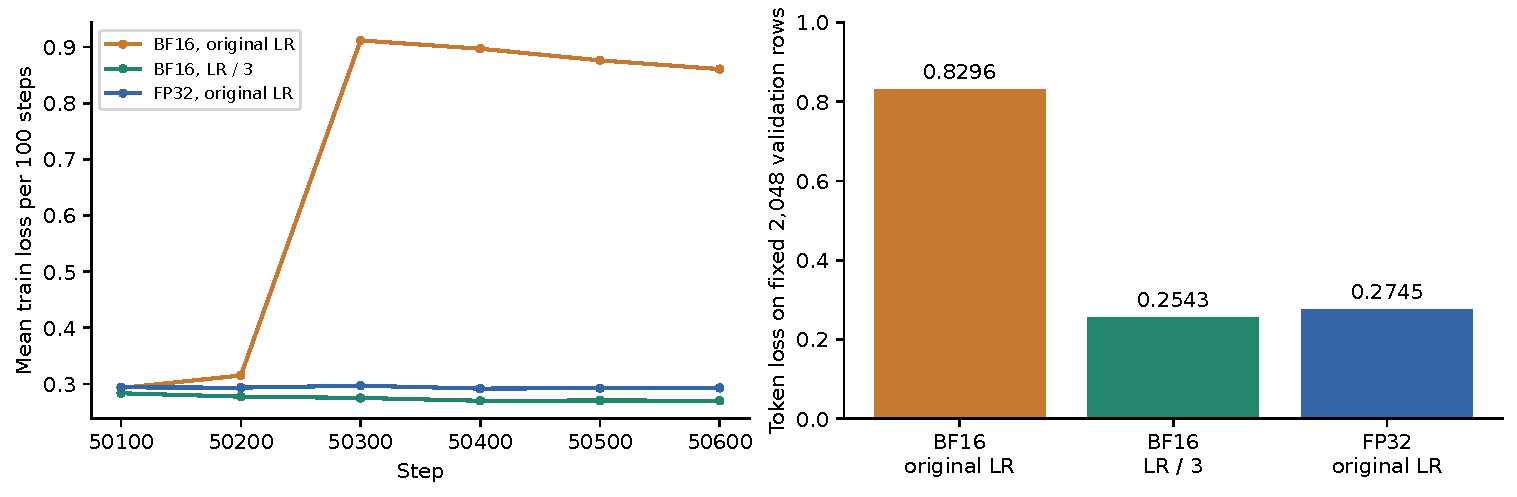
\includegraphics[width=\linewidth]{loss_diagnostic.pdf}
\caption{Диагностика модели 002. Слева --- средний train loss по 100 шагам,
справа --- token loss после 600 шагов на одной выборке 2048 примеров.
Эти короткие прогоны не доказывают долгосрочную устойчивость.}
\label{fig:diagnostic}
\end{figure}

Продолжение с checkpoint-50000 при LR $10^{-4}$ достигло суммарно
четырёх эпох и 362\,284 шагов. Лучший checkpoint-360000 имеет
validation token loss 0.1927033. На одном Test-002 последовательно
оценены checkpoint-50000, 90000 и 360000 (таблица~\ref{tab:old002}).

\begin{table}[htbp]
\centering\small\begin{tabular}{lrrr}
\toprule
Checkpoint & Greedy, \% & Beam 4, \% & Решено, beam 4 \\
\midrule
50000 & 60.21 & 63.03 & 6269/9946 \\
90000 & 68.09 & 69.69 & 6931/9946 \\
360000 & 71.66 & 72.84 & 7245/9946 \\
\bottomrule
\end{tabular}

\caption{Развитие модели 002 на неизменных 10\,000 строках Test-002,
9946 допустимых эталонов.}
\label{tab:old002}
\end{table}

\textbf{Вывод.} На диагностическом участке я смог устранить срыв,
уменьшив LR. После длительного продолжения я получил более высокое
качество генерации; финальный beam 4 добавил 118 решений к greedy
(+1.19 п.п.). После отправки этой модели в бота я получил
735/960 = 76.56\% на public. Это результат модели 002 на официальном
тесте, который я далее использовал для сравнения новых посылок.

\subsection{003: H100 и оптимизация цикла обучения}
Следующая конфигурация --- BART 10+10/d1024/FF4096, 303.18 млн
параметров, BF16, global batch 256 и LR $2\cdot10^{-4}$.
Исследовались расходы на padding, физический batch, fused AdamW
и \code{torch.compile}.
На коротком benchmark random/fused batch 128 дал около 614 примеров/с,
а группировка по длине и compile --- 1386 примеров/с;
padding уменьшился с 63.2\% до 25.5\%.
Начальная компиляция с прогревом заняла 96.3 секунды и исключена
из показателя throughput.

Дополнительный контроль на одинаковом checkpoint-7500, фиксированных
данных и трёх повторах сравнил attention (таблица~\ref{tab:attention}).
\begin{table}[htbp]
\centering\small
\begin{tabular}{llrr}
\toprule
Attention & Compile & Примеров/с, медиана & Пик allocated, ГиБ \\
\midrule
SDPA & нет & 1140.5 & 37.41 \\
FlashAttention-2 & нет & 1058.1 & 35.91 \\
FlashAttention-3 & нет & 1057.6 & 35.91 \\
SDPA & да & 1393.2 & 34.87 \\
FlashAttention-2 & да & 1041.7 & 33.44 \\
FlashAttention-3 & да & 1027.8 & 33.44 \\
\bottomrule
\end{tabular}
\caption{Training benchmark на H100: полный forward/backward/optimizer,
microbatch 128, accumulation 2, BF16.}
\label{tab:attention}
\end{table}

В штатном FA-адаптере обнаружено неверное применение encoder-маски
к decoder queries при unpadding cross-attention. В изолированном benchmark
адаптер исправлен и проверен по loss и градиентам; основной attention
не заменялся. Даже после этой проверки быстрее оказался SDPA с compile.
На свободной H100 batch 256 дал лишь +1.2\% throughput к 128$\times$2,
увеличив allocated memory с 34.87 до 65.79 ГиБ. Выбран 128$\times$2.

\textbf{Вывод.} Для своей модели с короткими последовательностями
я получил наибольшее ускорение от группировки по длине и SDPA+compile.
Их я оставил для продолжения поиска. Этот опыт показал мне, что
нужно измерять весь training pipeline: замена attention kernel сама
по себе не гарантирует ускорения. Здесь я сравнивал скорость обучения,
поэтому не использую эти числа как оценку качества генерации модели 003.

\subsection{004--005: глубина и learning rate на фиксированном бюджете}
Для быстрого отбора вместо полного обучения использован один миллион
фиксированных train, Val-20k, одна эпоха, global batch 256, seed 42,
warmup 5\% и cosine. BART-кандидаты различались глубиной и LR;
ширина оставалась 1024, FFN --- 4096.
В таблице~\ref{tab:h100} объединены восемь завершённых запусков двух серий.

\begin{table}[htbp]
\centering\small\begin{tabular}{lrrrr}
\toprule
E+D & LR & Парам., млн & Token loss & Время, с \\
\midrule
8+8 & 2e-04 & 244.39 & 0.394638 & 654.1 \\
8+12 & 2e-04 & 311.58 & 0.399215 & 828.0 \\
10+10 & 2e-04 & 303.18 & 0.436305 & 797.1 \\
10+10 & 1e-04 & 303.18 & 0.489001 & 796.1 \\
8+12 & 1e-04 & 311.58 & 0.496804 & 827.6 \\
12+8 & 1e-04 & 294.78 & 0.612622 & 764.1 \\
10+10 & 3e-04 & 303.18 & 0.850871 & 797.0 \\
12+8 & 2e-04 & 294.78 & 0.862528 & 762.7 \\
\bottomrule
\end{tabular}

\caption{Короткий поиск на H100: одинаковые 1M train и 20k validation.
Время --- wall time trial, а не время генерации.}
\label{tab:h100}
\end{table}

\begin{figure}[htbp]
\centering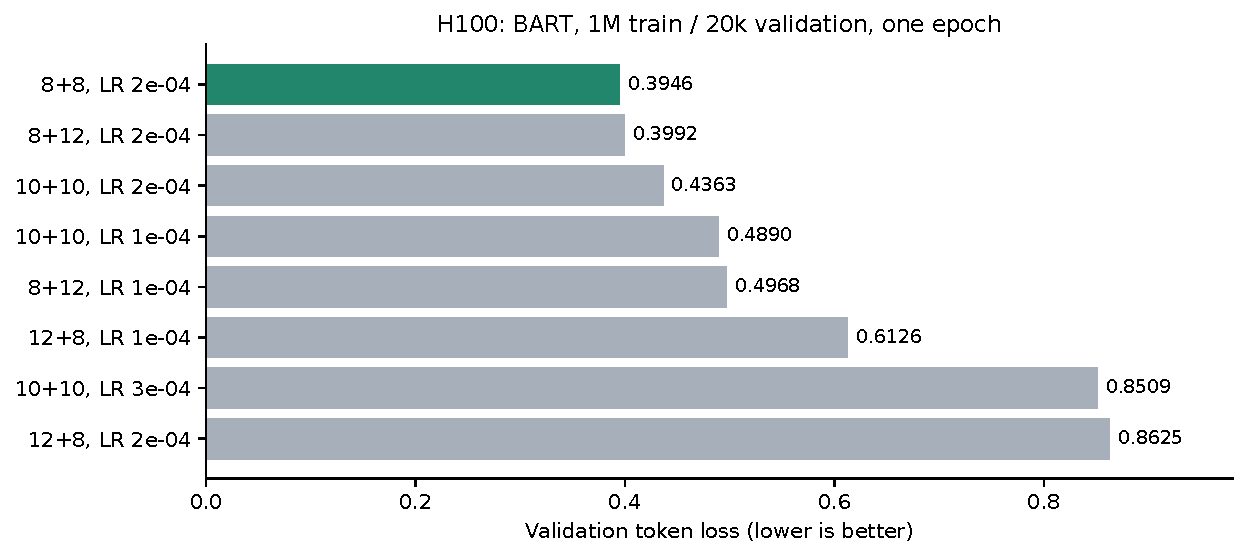
\includegraphics[width=.86\linewidth]{h100_sweep.pdf}
\caption{Validation token loss коротких BART-запусков. Меньшая модель
8+8 при LR $2\cdot10^{-4}$ оказалась лучшей в этом бюджете.}
\end{figure}

\textbf{Вывод.} Я не увидел преимущества более глубокого encoder 12+8.
Из проверенных вариантов я выбрал BART 8+8/d1024/FF4096
с LR $2\cdot10^{-4}$: он дал лучший loss при меньшем числе параметров
и меньшем времени. Я рассматривал это как отбор кандидата по раннему
обучению с одним seed, без вывода о превосходстве при любом бюджете.

\subsection{006--008: T5-style и копирование}
Проверена гипотеза, что другое устройство блоков или явное копирование
чисел из условия улучшат генерацию. Подготовленный H100-поиск T5
столкнулся с совместимостью TF32 API и Inductor; полноценным сравнимым
результатом T5 в этой части стали следующие завершённые Kaggle-запуски.
Отдельный smoke/preflight не рассматривается как измерение качества.

T5-style и Copy обучены на тех же 1M/20k, одну эпоху, LR
$2\cdot10^{-4}$, FP16, effective batch 256 на двух T4:
microbatch 16 на GPU, accumulation 8, gradient checkpointing.
Compile в окончательном Kaggle-рецепте отключён после исправления
ошибки runner, которая включала его через явно переданный backend.

\begin{table}[htbp]
\centering\small\begin{tabular}{lrrrr}
\toprule
Модель & Парам., млн & Token loss & Решено / 19886 & \pass{}, \% \\
\midrule
T5 & 247.31 & 1.012897 & 3333 & 16.7605 \\
Copy & 244.66 & 0.392547 & 10248 & 51.5337 \\
\bottomrule
\end{tabular}

\caption{Завершённые T5/Copy на Kaggle после одной эпохи.
Beam 4, 20\,000 validation, 19\,886 допустимых эталонов.}
\end{table}

Copy обучался около 2 ч 04 мин, T5 --- 2 ч 59 мин.
Генерация 20\,000 ответов на одной T4 для каждой модели заняла
1874.9 и около 4682.3 секунды соответственно.
\textbf{Вывод.} В этих настройках я получил у T5 заметно худший результат,
чем у Copy. Поэтому дальнейший отбор на A100 я сосредоточил на BART
и Copy. По одному LR, seed и одной эпохе я не делаю общего вывода
о возможностях T5. Скорость позднее обученного полного финалиста
я проверил отдельно на официальном тесте.


\section{Последовательные проверки на A100}

\subsection{Контроль BART против Copy}
Чтобы отделить эффект copy-head от различий оборудования и рецепта,
обе модели заново обучены на одной A100 в одинаковых условиях:
1M train, одна эпоха (3907 попыток шага), Val-20k, seed 42,
LR $2\cdot10^{-4}$, FP16, microbatch 128 и accumulation 2,
без gradient checkpointing и compile.

\begin{table}[htbp]
\centering\small\begin{tabular}{lrrrr}
\toprule
Модель & Token loss & Решено / 19886 & \pass{}, \% & Ошибки / 20k \\
\midrule
BART & 0.394293 & 10204 & 51.3125 & 368 \\
Copy & 0.393124 & 10203 & 51.3075 & 357 \\
\bottomrule
\end{tabular}

\caption{Сопоставимый контроль BART/Copy на A100. Ошибки кода считаются
по всем 20\,000 ответам; \pass{} --- по 19\,886 допустимым эталонам.}
\end{table}

BART решил на одну задачу больше: разница всего 0.0050 п.п.
Парно 9155 задач решены обеими моделями, 1049 --- только BART,
1048 --- только Copy. Заранее я решил выбирать более простой BART,
если Copy не превосходит его больше чем на 0.5 п.п.
\textbf{Вывод.} Я не увидел убедительного выигрыша от copy-head:
результаты отличались всего на одну задачу. Для следующих проверок
я оставил более простой BART.

\subsection{Повторение данных против разнообразия}
При неизменной архитектуре сравнивались два бюджета по четыре миллиона
предъявлений: исходный миллион, повторённый четыре раза, и четыре
миллиона различных исходных train-примеров. Обе модели обучались с нуля,
имели 15\,625 плановых попыток шага, одинаковые seed, batch, LR,
расписание и validation.

\begin{table}[htbp]
\centering\small\begin{tabular}{lrrr}
\toprule
Train / предъявления & Token loss & Решено / 19886 & \pass{}, \% \\
\midrule
1M $\times$ 4 & 0.267353 & 13445 & 67.6104 \\
4M различных & 0.250444 & 13657 & 68.6765 \\
\bottomrule
\end{tabular}

\caption{Сравнение числа различных train-примеров при одном бюджете
предъявлений. Протокол оценки: beam 4, LP 1.0, max 256.}
\label{tab:diversity}
\end{table}

\begin{figure}[htbp]
\centering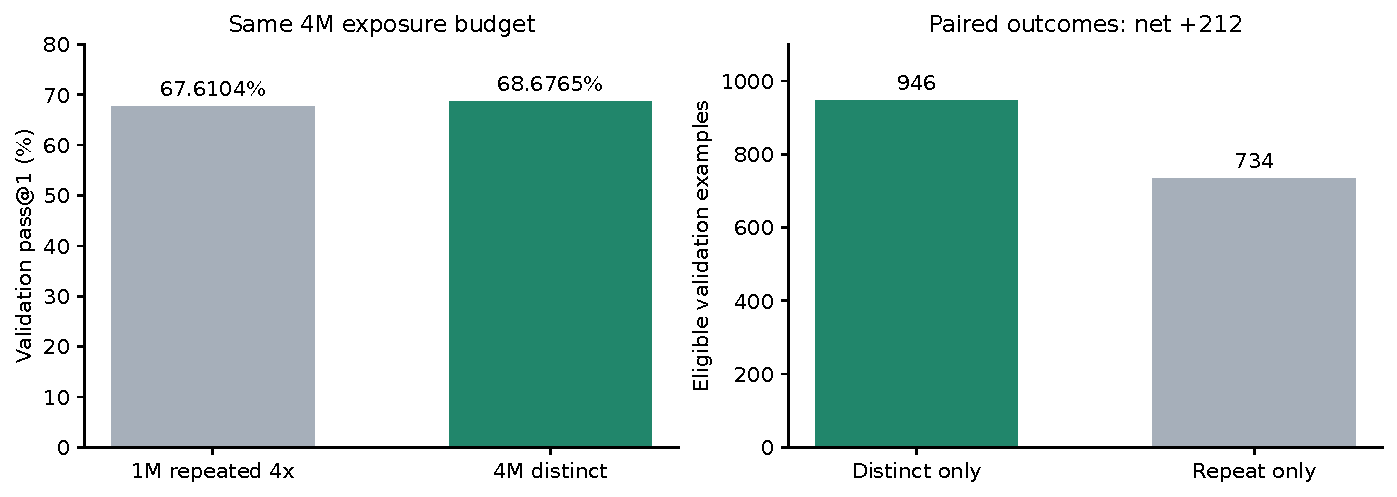
\includegraphics[width=\linewidth]{data_diversity.pdf}
\caption{Разнообразие данных: качество и парные несовпадения.
Обе модели решили 12\,711 задач; 5495 не решила ни одна.}
\end{figure}

Distinct4m решил дополнительно 212 задач (+1.0661 п.п.):
946 решены только им и 734 --- только Repeat4m.
Количество ошибок кода уменьшилось со 113 до 70 на 20\,000 ответов.
Это непосредственное основание расширить обучение на все исходные train.

Первый Repeat4m был прерван из-за взаимодействия собственного guard
с native AMP. После диагностики я продолжил его из checkpoint-14000
в отдельной папке, сохранив результаты первой попытки.
Был обработан один overflow в resumed-сессии Repeat4m
и два в Distinct4m. Поэтому равенство плановых попыток не гарантирует
равенства числа успешных обновлений. Агрегат \code{train_loss} после
resume не интерпретировался как среднее всего эксперимента.

\textbf{Вывод.} При том же бюджете предъявлений я получил более высокое
качество на различных примерах, чем при повторении одного миллиона.
Этот результат стал для меня основанием перейти к полному train.
Пока я проверил это только с одним seed и бюджетом, поэтому не переношу
наблюдение автоматически на другие объёмы и модели.

\subsection{Аудит ошибок и качества эталонов}
Выполнен ручной семантический разбор 200 случайных допустимых ошибок
Distinct4m и 200 примеров исходного train. Все 400 программ синтаксически
корректны и содержат \code{solve()}, что само по себе не подтверждает
их содержательную правильность.

В 200 train-примерах отмечены 48 несоответствий условие--код,
2 возврата неопределённой переменной, 29 проблем формулировки и 3 прочих
замечания; в 118 конкретный дефект не найден.
В выбранных 200 validation-ошибках помечены 125 сомнительных эталонов,
34 неоднозначных или неполных условия, 2 соглашения о точности;
в 39 конкретная проблема эталона не найдена.

Например, один эталон вычитает вес постороннего рюкзака из веса
постиранной одежды; два train-эталона присваивают результат одной
переменной, но возвращают неопределённую \code{result}.
Два первоначальных замечания об отсутствии \code{import math} сняты:
фактический evaluator предоставляет \code{math} в окружении.

\textbf{Вывод.} При разборе примеров с помощью Codex я увидел,
что часть ошибок метрики связана с самим корпусом и не обнаруживается
синтаксической проверкой. Я использовал эти отметки для понимания ошибок,
но не считаю их измеренной долей шума во всём датасете:
validation-примеры выбирались среди неуспехов модели.
По результатам аудита я не менял таргеты и знаменатель \pass{}
и не создавал дополнительные данные.

\subsection{Выбор beam и length penalty}
На первых 2000 строках той же Val-20k сравнены пять вариантов декодирования
Distinct4m. Допустимы 1988 эталонов; seed и checkpoint фиксированы.

\begin{table}[htbp]
\centering\small\begin{tabular}{rrrrrr}
\toprule
Beam & LP & Batch & Решено / 1988 & \pass{}, \% & A100, с \\
\midrule
2 & 1.0 & 64 & 1365 & 68.6620 & 42.55 \\
4 & 1.0 & 64 & 1378 & 69.3159 & 53.63 \\
8 & 1.0 & 32 & 1376 & 69.2153 & 95.47 \\
4 & 0.8 & 64 & 1378 & 69.3159 & 50.85 \\
4 & 1.2 & 64 & 1378 & 69.3159 & 51.74 \\
\bottomrule
\end{tabular}

\caption{Подбор декодирования на A100. Для beam 8 batch уменьшен
до 32; у остальных вариантов batch 64.}
\label{tab:decoding}
\end{table}

\begin{figure}[htbp]
\centering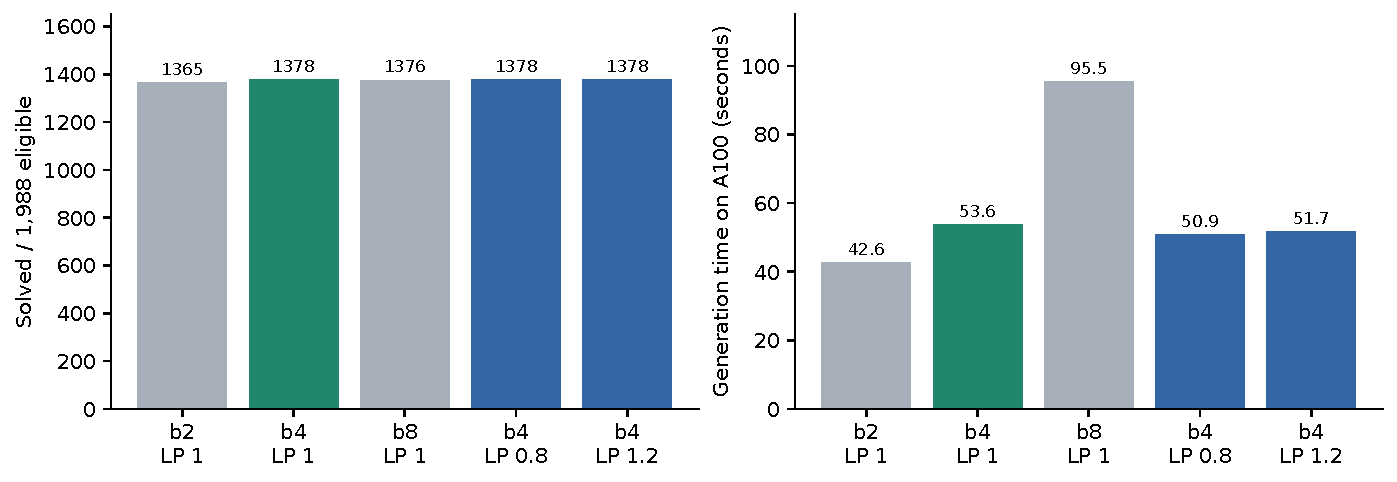
\includegraphics[width=\linewidth]{decoding.pdf}
\caption{Количество решённых задач и стоимость генерации на subset 2k.
Зелёным выделен выбранный beam 4 / LP 1.0.}
\end{figure}

По заранее заданному правилу выбирается больше решённых задач,
при равенстве --- меньший beam, затем LP ближе к 1.0.
Выбран beam 4 / LP 1.0. На полной Val-20k подтверждены
13\,657/19\,886 = 68.6765\%; все предсказания и pass-флаги совпали
с прежней оценкой Distinct4m. Генерация заняла 464.44 секунды на A100.
\textbf{Вывод.} Я оставил beam 4 / LP 1.0: увеличение beam до 8
не улучшило результат на subset, но увеличило время генерации.
От изменения LP я также не получил выигрыша по \pass{}.

\subsection{Полное обучение выбранного BART}
На основании предыдущих проверок BART 8+8/d1024/FF4096 обучен с нуля
на 11\,593\,060 train. Использованы неизменный BPE8000,
полные 118\,302 validation, FP16, seed 42, LR $2\cdot10^{-4}$,
cosine с warmup 5\%, global batch 256 = 128$\times$2,
лимиты 256/256, без compile и gradient checkpointing.
Validation и resumable checkpoint сохранялись каждые 5000 шагов.
Рецепт допускал четыре эпохи и early stopping с patience 5 по token loss.

\begin{table}[htbp]
\centering\small
\begin{tabularx}{\linewidth}{lX}
\toprule
Показатель & Результат \\
\midrule
Завершение & 23 октября, 16:26:37 МСК; exitcode 0 \\
Бюджет & 4 эпохи, 181\,144 плановых попытки шага \\
Время trial & 53\,940.95 с, около 14 ч 59 мин \\
Лучший checkpoint & 180\,000; validation token loss 0.1910213150 \\
Повторная оценка экспорта & 0.1910215739 на 7\,970\,835 целевых токенах \\
Пиковая allocated memory & 32.55 ГиБ на A100 80GB PCIe \\
Early stopping & Не сработал; достигнут предел эпох \\
AMP & 66 обработанных overflow; сохранённые loss конечны \\
\bottomrule
\end{tabularx}
\caption{Завершённое полное обучение. Повторная оценка лучших весов
не является оценкой последних обновлённых весов.}
\end{table}

\begin{figure}[htbp]
\centering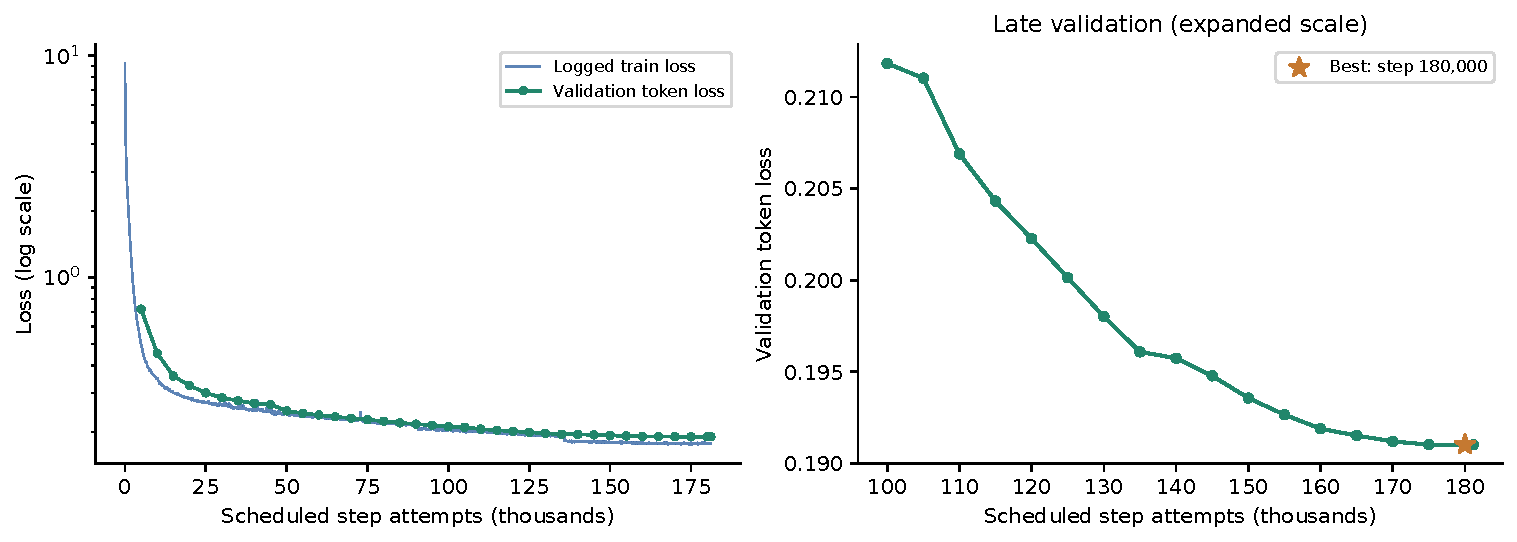
\includegraphics[width=\linewidth]{full_training.pdf}
\caption{Полное обучение BART. Слева --- обзор loss в логарифмическом
масштабе, справа --- поздняя validation с увеличенным масштабом.
Линия validation относится к весам соответствующих шагов; последняя
повторная оценка восстановленных лучших весов в неё не подставляется.}
\label{fig:full}
\end{figure}

Финальный экспорт побитово совпал с checkpoint-180000;
все 344 сохранённых тензора конечны. Лучший и последний checkpoint
с optimizer, scheduler, scaler и RNG оставлены на сервере.
Локально сохранены небольшие метрики, конфигурации и графики.

\textbf{Вывод.} Я довёл выбранную конфигурацию до четырёх эпох
и получил token loss 0.1910 на полной validation без срыва обучения.
После экспорта я отдельно проверил качество генерации и время
на официальном наборе задач на T4.

\subsection{Качество полной модели на прежней validation}
Финальный экспорт checkpoint-180000 оценён на той же Val-20k,
что Distinct4m: beam 4, LP 1.0, максимум 256 новых токенов,
один итоговый кандидат, те же 19\,886 допустимых эталонов.
Проверены идентичность всех строк и эталонных результатов, SHA256 весов,
счётчики и сохранённые pass-флаги.

\begin{table}[htbp]
\centering\small\begin{tabular}{lrrr}
\toprule
Модель / бюджет & Решено / 19886 & \pass{}, \% & Ошибки / 20k \\
\midrule
Distinct4m / 4M & 13657 & 68.6765 & 70 \\
Полный train / 4 эпохи & 14775 & 74.2985 & 32 \\
\bottomrule
\end{tabular}

\caption{Короткий Distinct4m и полностью обученный BART на одной
Val-20k. Бюджеты обучения различаются; это сравнение итоговых
конфигураций, а не опыт с одинаковым числом предъявлений.}
\label{tab:fullquality}
\end{table}

Полная модель решила дополнительно 1118 задач (+5.6220 п.п.).
Парно 13\,101 задача решена обеими моделями, 1674 --- только полной,
556 --- только Distinct4m, 4555 не решила ни одна.
Доля ошибок кода снизилась с 0.35\% до 0.16\% от всех 20\,000 ответов;
лимит длины достигнут в 9 случаях вместо 15.
Генерация полной выборки на A100 заняла 466.75 секунды,
исполнение --- 245.29 секунды.

\textbf{Вывод.} По сравнению с коротким Distinct4m я получил более высокое
качество на неизменной validation. Эту выборку я использовал
для мониторинга loss и выбора checkpoint, поэтому отдельно проверил
новую модель в официальном checker. Public 76.56\% старой модели 002
я не сравниваю напрямую с validation 74.2985\% новой модели.

\subsection{Фактический финалист на одной T4}
В приватном Colab-сеансе выполнен полный прогон официальных 1919
условий на одной Tesla T4. SHA256 весов совпал с экспортом лучшего
checkpoint-180000; порядок всех вопросов закреплён отдельно.
Использованы FP16, beam 4, LP 1.0, KV-cache, группировка по длине,
batch 128 и максимум 256 новых токенов. Входные вопросы не обрезались,
исполнение сгенерированного кода в замер не входило.

\begin{table}[htbp]
\centering\small
\begin{tabularx}{\linewidth}{lX}
\toprule
Показатель & Результат \\
\midrule
GPU / число устройств & Tesla T4 / 1 \\
Модель & Лучший BART 8+8/d1024, checkpoint-180000 \\
Официальные условия & 1919, без открытых эталонных ответов \\
Декодирование & FP16, beam 4, LP 1.0, batch 128, max 256 \\
Время инференса & 165.07 с внутри pipeline; 165.11 с внешний wall time \\
Загрузка весов, отдельно & 4.30 с \\
Пик allocated memory & 8.07 ГиБ \\
Пустые ответы / достижение лимита & 0 / 0; все ответы завершены EOS \\
Окружение & PyTorch 2.11.0+cu130, Transformers 5.10.2 \\
\bottomrule
\end{tabularx}
\caption{Измеренный протокол официальной генерации фактическим
финалистом на одной T4.}
\end{table}

Таймер включает токенизацию, сортировку по длине, переносы, генерацию,
декодирование и сборку ответов. Загрузка checkpoint, установка зависимостей
и запись файлов исключены; отдельного generation warmup не было.
Внешнее wall time также меньше 180 секунд, запас --- около 14.9 секунды.
Этот результат подтверждает выполнение ограничения в измеренном runtime;
скорость может отличаться между Colab-сеансами.

Я отправил боту файл из 1919 ответов. Результат и сравнение
с моей предыдущей посылкой приведены далее.

\subsection{Public: сравнение с прежней полной моделью 002}
\begin{table}[htbp]
\centering\small\begin{tabular}{>{\raggedright\arraybackslash}p{.30\linewidth}>{\raggedright\arraybackslash}p{.28\linewidth}>{\raggedright\arraybackslash}p{.28\linewidth}}
\toprule
Параметр & Прежняя 002 & Новая полная \\
\midrule
Encoder + decoder & 8+8 & 8+8 \\
Hidden / FFN & 768 / 3072 & 1024 / 4096 \\
Параметры, млн & 139.25 & 244.39 \\
Train / эпохи & 11\,593\,060 / 4 & 11\,593\,060 / 4 \\
BPE / seed & 8000 / 42 & 8000 / 42 \\
Global batch & 128 & 256 \\
LR & $3\cdot10^{-4}$; после 50k $10^{-4}$ & $2\cdot10^{-4}$ \\
Точность обучения & BF16 & FP16 \\
Лучший checkpoint & 360000 & 180000 \\
Token loss Val-full & 0.1927033 & 0.1910213 \\
Beam / max tokens & 4 / 256 & 4 / 256 \\
Public & 735/960 (76.5625\%) & 729/960 (75.9375\%) \\
\bottomrule
\end{tabular}

\caption{Предыдущая официальная модель 002 и новая полная модель.
Public сравнивается с public на 960 задачах; private ещё неизвестен.}
\label{tab:publiccomparison}
\end{table}

У обеих моделей BART 8+8, один и тот же BPE8000,
полный подготовленный train и четыре эпохи. Новая модель обучена
\emph{с нуля}, а не продолжением весов 002; она шире, имеет больший FFN
и около 244 млн параметров вместо 139 млн.
Одновременно изменены global batch, LR и точность обучения.
Поэтому это сравнение двух рецептов, а не изолированная абляция ширины.
Вдвое меньшее число шагов нового запуска связано с удвоением global batch
и само по себе не означает вдвое меньшее число предъявленных примеров.

По сводке бота доля ошибок исполнения снизилась с 0.21\% до 0.10\%,
но доля неверных ответов выросла с 23.23\% до 23.96\%.
Отсутствующего кода и синтаксических ошибок в обеих public-сводках нет.
Агрегаты не показывают, какие задачи новая модель исправила или потеряла:
шесть --- чистая разница числа решений, а не число изменившихся ответов.

\textbf{Вывод.} На public я получил на шесть решений меньше
($-0.625$ п.п.), хотя token loss на полной validation немного снизился.
Для меня это показало, что больший размер модели и меньший loss
ещё не гарантируют улучшения официального результата.
Прирост 68.6765\% $\to$ 74.2985\% я получил относительно короткого
Distinct4m, а не прежней полной модели 002.
\pending{Какая из двух полных моделей окажется лучше на private,
я пока не знаю.}


\section{Ограничения и промежуточные выводы}

По ходу работы я несколько раз менял дальнейшие планы по результатам
коротких проверок. После сравнения с greedy я стал использовать beam 4.
Для модели 002 я снизил LR после воспроизведения срыва обучения.
В поиске на H100 я выбрал BART 8+8/d1024, который в этом бюджете
обучался лучше более глубоких вариантов. На A100 я не увидел выигрыша
от copy-head, зато получил +1.0661 п.п. при замене повторяющихся
данных четырьмя миллионами различных примеров.

После полного обучения выбранного BART я получил 74.2985\% на той же
validation и уложился в ограничение T4: 165.1 секунды на официальный test.
Однако на public моя прежняя полная модель 002 осталась лучше:
735/960 против 729/960 у новой. Поэтому я не считаю более широкий BART
безусловным улучшением своего решения. Рост относительно короткого
Distinct4m не означал роста относительно предыдущей официальной посылки.

При интерпретации результатов я учитываю следующие ограничения:
\begin{itemize}
\item В основных сравнениях использован один seed. Разница одной задачи
между BART и Copy не устанавливает превосходство архитектуры.
\item Ранняя сходимость на 1M не определяет порядок моделей после полного
обучения; архитектуры оценивались в конкретном LR и бюджете.
\item Validation использовалась для выбора моделей, checkpoint и decoding.
Это не независимая итоговая оценка обобщения.
\item Public новой модели оказался ниже public модели 002 на шесть решений.
По одним агрегатам нельзя восстановить парные изменения ответов
или сделать вывод о качестве на пока закрытой private-половине.
\item Разбиение по строкам допускает одинаковые и близкие условия
в разных частях; зависимость примеров не учтена оценкой метрики.
\item Эталонные программы содержат смысловые дефекты. Согласие с их
выводом отличается от правильности относительно условия.
\item Потери на Val-20k и Val-full имеют разные наборы примеров;
их численные значения нельзя использовать как прямое парное сравнение.
\item Ограничение T4 проверено отдельным реальным прогоном финалиста,
а не пересчётом A100 timing или training throughput. Это один замер;
запас около 14.9 секунды не гарантирует то же время в любом runtime.
\end{itemize}

\section{Как я использовал ИИ-агентов}
Я формулировал цели, задавал ограничения и выбирал направления
экспериментов. GPT/Codex я использовал для обсуждения гипотез,
написания и проверки кода, подготовки запусков, анализа журналов
и ведения отчёта. Например, я поручил Codex реализовать общий pipeline,
подготовить сравнения моделей и собрать метрики из сохранённых результатов.
В таблице я перечислил основные задачи агентов и то, как они помогли
мне принимать решения.

\begin{table}[htbp]
\centering\small
\begin{tabularx}{\linewidth}{>{\raggedright\arraybackslash}p{.20\linewidth}YY}
\toprule
Задача агента & Что было сделано & Влияние на решение \\
\midrule
Подготовка данных & Загрузка, очистка комментариев, разбиения, BPE,
контроль labels и padding & Единый воспроизводимый pipeline для моделей \\
Модели и обучение & BART/T5/Copy, DDP, resume, token-normalized loss,
проверки сохранения и генерации & Возможность сопоставлять архитектуры
без переписывания основного pipeline \\
Диагностика и ревью & Воспроизведение срыва 002, проверка LR,
масок cross-attention, compile и AMP & Выбор стабильного LR,
исправление ошибок до интерпретации результатов \\
Эксперименты & Подготовка конфигураций, preflight, мониторинг,
сбор метрик и парных исходов & Быстрый короткий отбор перед полным
обучением; сохранение фактов при сбоях \\
Разбор результатов & Аудит 200+200, контроль эталонов,
таблицы, графики и этот LaTeX-черновик & Уточнение ограничений метрики
и причин выбора следующего эксперимента \\
\bottomrule
\end{tabularx}
\caption{Использование агентов по журналу проекта.}
\end{table}

Я опирался на тесты, короткие реальные прогоны и сохранённые метрики,
которые агент готовил для проверки предложений. Отдельное ревью помогло
найти, например, скрытое включение compile и ошибочную интерпретацию
отсутствующего \code{import math}. При разборе шума я использовал
суждения агента как подсказки для анализа примеров, но не как основание
для создания новых таргетов или изменения знаменателя \pass{}.
Выбор следующего эксперимента и решения о длительном обучении
я оставлял за собой.

\section{Что добавить в следующую версию}
\begin{enumerate}
\item \pending{После открытия private добавить результаты обеих моделей,
если они будут доступны, и уточнить итоговый вывод о качестве.}
\item При необходимости сравнить старую полную модель 002 с новой
полной моделью на одном согласованном отложенном наборе;
разные public и validation метрики не заменяют такое сравнение.
\item Я хочу дополнить текст показательными примерами программ
и сократить вспомогательные детали, чтобы яснее объяснить логику экспериментов.
\end{enumerate}

\clearpage
\appendix
\section{Источники чисел и воспроизведение рисунков}
Журнал работы находится в \code{README.md}, первичные результаты ---
в каталоге \code{reports/}. Сопровождающий \path{report/source_manifest.json}
фиксирует SHA256 и размер JSON-файлов, из которых построены таблицы и рисунки.
Скрипт \path{report/build_figures.py} читает только сохранённые результаты:
он не запускает обучение, инференс или выполнение программ.

Для обновления иллюстраций из корня репозитория используется команда:
\begin{quote}\small\code{python3 report/build_figures.py}\end{quote}
Исходник документа разделён на
файлы в \code{report/sections/}; точка входа --- \code{report/main.tex}.
Сохранённые проверки Stage2 и Stage4 подтверждают идентичность
validation и эталонов, а финальная сводка полного обучения --- exitcode 0
и соответствие экспорта лучшему checkpoint.
Предварительные планы и незавершённые попытки в этом отчёте явно
отделены от фактически завершённых экспериментов.


\begingroup\small
\begin{thebibliography}{9}
\setlength{\itemsep}{2pt}
\bibitem{assignment}
HSE NLP, домашнее задание 2: «Генерация кода», 2026.
\url{https://github.com/ashaba1in/hse-nlp/blob/2026/homeworks/hw2_code_generation.md}.

\bibitem{dataset}
SlavaYus. \emph{tinysms\_qa\_12m}, Hugging Face dataset.
\url{https://huggingface.co/datasets/SlavaYus/tinysms_qa_12m}.

\bibitem{bart}
Lewis M. et al. \emph{BART: Denoising Sequence-to-Sequence Pre-training
for Natural Language Generation, Translation, and Comprehension}, 2019.
\url{https://arxiv.org/abs/1910.13461}.

\bibitem{t5}
Raffel C. et al. \emph{Exploring the Limits of Transfer Learning with a
Unified Text-to-Text Transformer}, 2019.
\url{https://arxiv.org/abs/1910.10683}.

\bibitem{pointer}
See A., Liu P. J., Manning C. D. \emph{Get To The Point: Summarization
with Pointer-Generator Networks}. ACL, 2017, pp. 1073--1083.
\url{https://aclanthology.org/P17-1099/}.
\end{thebibliography}
\endgroup

\end{document}
